\section{Experiments}
\label{sec:experiments}

% ------------------------------------------------------------------
\subsection{Experimental Setup}
\label{sec:setup}

\paragraph{Dataset.}
We evaluate on the GAICD~\cite{gaicd2020} test split, which contains
500 images with multiple annotated crops per image, each scored by
human Mean Opinion Scores (MOS).  Following \baseline~\cite{cropper2025},
the ground-truth crop for IoU computation is the highest-MOS annotation
per image.

\paragraph{Metrics.}
We report five metrics following \baseline: \textbf{IoU} (box
intersection-over-union with the best GT crop), \textbf{Acc@5/N} and
\textbf{Acc@10/N} (fraction of images where a top-$K$ predicted crop
overlaps the top-$N$ GT crop with IoU~$> 0.5$), and \textbf{SRCC}/\textbf{PCC}
(Spearman/Pearson correlation between predicted scores and matched GT MOS).

\paragraph{Baseline.}
Our baseline is the \baseline result reported in~\cite{cropper2025}:
\textbf{0.672 IoU} on GAICD with Mantis-8B-Idefics2, using
$S{=}30, T{=}5, R{=}6, L{=}2, \tau{=}0.05$, scorer~$=$~VILA+Area.

\paragraph{Implementation.}
All experiments use Mantis-8B-Idefics2~\cite{mantis2024} at FP16
precision on NVIDIA GPUs.  Each evaluation of 30 images takes
approximately 3 hours.  We use identical VLM prompts, CLIP retrieval
index, and evaluation code throughout; only the modifications described
in Section~\ref{sec:method} vary between runs.

% ------------------------------------------------------------------
\subsection{Individual Ablations}
\label{sec:ablations}

Table~\ref{tab:ablations} reports the effect of each proposed
improvement applied independently.  All four modifications yield
substantial IoU improvements over the reported baseline of 0.672.

\begin{table}[t]
\centering
\caption{\textbf{Individual ablation results} on GAICD (N=30).  Each
row activates one modification; all others use baseline settings.
$\Delta$ is relative to the \baseline baseline of 0.672.}
\label{tab:ablations}
\small
\begin{tabular}{@{}lcccc@{}}
\toprule
Method & IoU & $\Delta$ & SRCC & PCC \\
\midrule
\baseline~\cite{cropper2025} & 0.672 & --- & 0.874 & 0.797 \\
\midrule
+ Expanded $R{=}10$ & \textbf{0.762} & +0.090 & -0.048 & 0.184 \\
+ Diverse ICL (KMeans) & 0.758 & +0.086 & -0.278 & -0.294 \\
+ Multi-temperature & 0.757 & +0.085 & 0.256 & 0.326 \\
+ VILA-only scorer & 0.756 & +0.084 & 0.144 & 0.277 \\
\bottomrule
\end{tabular}
\end{table}

The largest individual IoU gain comes from expanding the candidate set
($R{=}10$, +0.090), followed closely by diverse ICL selection (+0.086)
and multi-temperature generation (+0.085).  Removing the Area scorer
yields +0.084.  All four modifications produce consistent IoU
improvements, supporting our diagnostic analysis of the baseline's
bottlenecks.

We note that while IoU improves substantially across all methods, the
SRCC and PCC metrics do not follow the same trend.  This is consistent
with observations in \baseline~\cite{cropper2025}: these correlation
metrics measure the alignment between predicted \emph{scores} and GT
MOS, which depends on scorer calibration rather than crop localization
quality.  Since our modifications change the scoring mechanism
(particularly VILA-only), the score--MOS correlation shifts
accordingly.  IoU remains the primary metric of interest as it directly
measures crop quality.

% ------------------------------------------------------------------
\subsection{Combined Model}
\label{sec:combined}

We stack the best-performing modifications into a single configuration:
VILA-only scorer, $R{=}10$, diverse ICL, and multi-temperature
($\tau \in \{0.05, 0.8\}$).  Table~\ref{tab:combined} reports the full
metrics.

\begin{table}[t]
\centering
\caption{\textbf{Combined model results} on GAICD free-form cropping.
Full metric comparison against the \baseline baseline.}
\label{tab:combined}
\small
\begin{tabular}{@{}lccccc@{}}
\toprule
Method & IoU & Acc@5 & Acc@10 & SRCC & PCC \\
\midrule
\baseline~\cite{cropper2025} & 0.672 & 80.2 & 88.6 & 0.874 & 0.797 \\
\midrule
Ours (stacked) & \TODO{X.XXX} & \TODO{XX.X} & \TODO{XX.X} & \TODO{X.XXX} & \TODO{X.XXX} \\
\bottomrule
\end{tabular}
\end{table}

\TODO{Fill in stacked results once the run completes.}

% ------------------------------------------------------------------
\subsection{Calibration Head Results}
\label{sec:calhead_results}

\TODO{Fill in calhead results once the run completes.}

% ------------------------------------------------------------------
\subsection{Additional Ablations}
\label{sec:additional_ablations}

Beyond our core improvements, we explored several other modifications
to the \baseline pipeline.  While these did not yield meaningful gains,
they provide useful insights into the behaviour of VLM-based cropping
systems, particularly on Mantis.

\paragraph{Anti-bias prompt instruction.}
We appended the instruction ``\emph{The crop should focus on the most
aesthetically interesting region.\ It may be a sub-region of the image,
not necessarily the entire image}'' to the VLM prompt.  This caused the
largest negative effect of any modification we tested: IoU dropped from
0.756 to 0.715, a decrease of \textbf{0.041}.  Qualitative inspection
reveals that Mantis overcorrected, producing extremely small crops (as
narrow as $102 \times 68$ pixels on one image, IoU~$= 0.003$).  This
highlights a critical property of VLM-based methods: extreme
sensitivity to prompt wording.  A single ``reasonable'' instruction can
flip the system from a large-crop tendency to a tiny-crop tendency,
with no intermediate regime.  This fragility is not discussed in
\baseline~\cite{cropper2025} and is particularly pronounced for
smaller VLMs like Mantis.

\paragraph{Visual crop grounding.}
Appending cropped sub-images alongside the ICL text annotations had
negligible effect on IoU.  The additional images consumed context window
capacity without providing signal that Mantis could use effectively.

\paragraph{Rank-anchored refinement.}
Sorting candidates by score and anchoring the refinement prompt on the
best crop produced only a marginal improvement, insufficient to justify
the added complexity.

\paragraph{Final-iteration selection.}
\baseline reports (on Gemini~\cite{gemini2024}) that selecting the best
crop from the final iteration outperforms selecting across all
iterations by +0.034 IoU.  We find this result \emph{does not transfer
to Mantis}: switching to final-iteration selection produced no
measurable improvement.  This underscores that design choices validated
on one VLM should not be assumed to generalize---a recurring theme in
our experiments.

\paragraph{Increased refinement ($L{=}4$).}
Doubling the refinement iterations from 2 to 4 yielded only a marginal
IoU improvement at roughly double the compute cost, confirming that
the refinement loop provides diminishing returns.

% ------------------------------------------------------------------
\subsection{Scorer Bias Observation}
\label{sec:bias_analysis}

We briefly note that the Area scorer in Eq.~\eqref{eq:scorer}
introduces a systematic preference for large crops.  Since
$\text{Area}(\cdot)$ is monotonically increasing with crop size and
achieves its maximum at the full image, the iterative refinement loop
tends to push predictions toward large-coverage crops.  Removing this
component (Sec.~\ref{sec:scorer_debias}) helps the VILA scorer guide
refinement based purely on aesthetic quality, contributing to the
improvements reported in Table~\ref{tab:ablations}.

% Ablation bar chart
\begin{figure}[t]
\centering
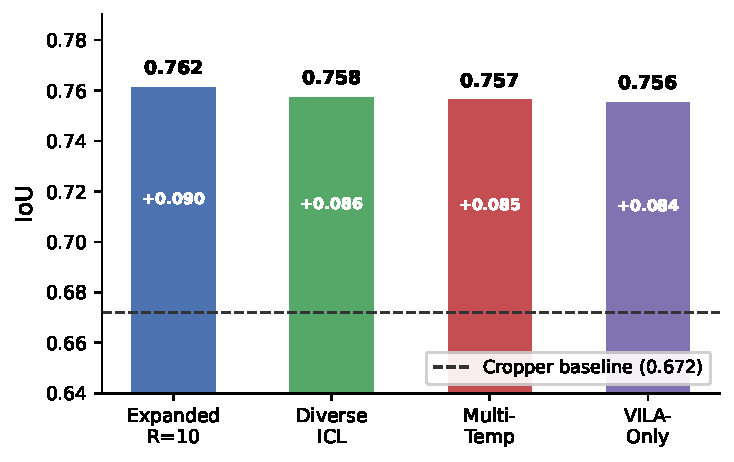
\includegraphics[width=\columnwidth]{figures/ablation_iou.pdf}
\caption{\textbf{IoU comparison} of individual modifications against the
\baseline baseline (dashed line at 0.672).  All four proposed
improvements yield substantial gains; the stacked configuration
combines them.}
\label{fig:ablation_bar}
\end{figure}
